\documentclass[11pt,a4paper]{article}

% --- Packages ---
\usepackage[utf8]{inputenc}
\usepackage[T1]{fontenc}
\usepackage{amsmath,amssymb,amsthm}
\usepackage{graphicx}
\usepackage{booktabs}
\usepackage{subcaption}
\usepackage[colorlinks=true,linkcolor=blue,citecolor=blue,urlcolor=blue]{hyperref}
\usepackage[round]{natbib}
\usepackage[margin=2.5cm]{geometry}
\usepackage{xcolor}
\usepackage{algorithm}
\usepackage{algpseudocode}
\usepackage{multirow}
\usepackage{enumitem}
\usepackage{float}

% --- Custom commands ---
\newcommand{\vt}{v_\theta}
\newcommand{\xt}{x_t}
\newcommand{\ut}{u_t}
\newcommand{\R}{\mathbb{R}}
\newcommand{\E}{\mathbb{E}}
\newcommand{\Var}{\mathrm{Var}}
\DeclareMathOperator*{\argmin}{arg\,min}
\DeclareMathOperator{\softmax}{softmax}

% --- Title ---
\title{\textbf{Variance-Reduction Composition in Conditional Flow Matching:\\From 2D Experiments to CIFAR-10}}
\author{
  Sacha Leiderr \and Amine Soukane
}
\date{Master 2 Deep Learning --- March 2026}

\begin{document}

\maketitle

\begin{abstract}
Conditional Flow Matching (CFM) trains continuous normalizing flows via simulation-free velocity regression, but the single-sample conditional target induces high gradient variance. Three independent techniques address this: minibatch optimal-transport coupling (BatchOT), importance-weighted marginal velocity targets (StableVM), and antithetic temporal sampling with consistency regularization (TPC). We investigate whether these techniques compose additively through two complementary studies. On 2D synthetic distributions, we confirm that OT-type paths produce straighter trajectories and superior low-NFE robustness. On CIFAR-10, we cross the three axes in a $2^3$ factorial ablation: only one of eight cells converged---BatchOT with standard CFM and uniform sampling (FID~18.4). The other seven diverged or oscillated due to dimension-dependent numerical instabilities invisible in 2D. These negative results reveal that StableVM's importance weights scale catastrophically with dimension ($d{=}3072$), TPC's consistency penalty causes gradient explosions, and the three axes are not additive. BatchOT alone is the single most impactful variance-reduction technique.
\end{abstract}

\section{Introduction}

Generative modeling has undergone a paradigm shift with the success of diffusion models \citep{ho2020denoising, song2021scorebased}, which learn to reverse a noise-corruption process to generate samples. While highly effective, these models require simulating stochastic differential equations (SDEs) during both training and sampling, leading to computational overhead and sensitivity to discretization.

\textbf{Flow Matching} (FM), introduced by \citet{lipman2023flow}, offers an alternative based on continuous normalizing flows (CNFs). Instead of learning to reverse a diffusion process, FM directly regresses a neural velocity field $\vt(x, t)$ against a target vector field that transports a simple prior $p_0$ (e.g., standard Gaussian) to the data distribution $p_1$. The key advantage is simulation-free training: no ODE must be solved during the training loop, only at sampling time.

\textbf{Conditional Flow Matching} (CFM) makes FM practical by decomposing the intractable marginal vector field into tractable conditional terms. Each training sample defines a conditional probability path from noise to data, and the velocity field is trained to match the conditional vector field along this path. This yields a simple regression loss that is unbiased for the marginal FM objective.

\paragraph{The variance problem.} While unbiased, the CFM loss has high variance because each training step sees only a single conditional vector field sample. This variance manifests as noisy gradients, slower convergence, and degraded sample quality at low numbers of function evaluations (NFE). Three independent research directions have proposed solutions along different axes:

\begin{enumerate}[leftmargin=*]
    \item \textbf{Coupling} --- replacing independent noise--data pairing ($x_0 \sim p_0$ independent of $x_1 \sim p_1$) with minibatch optimal transport (BatchOT), which finds low-cost pairings within each minibatch \citep{tong2024improving}. This straightens trajectories and reduces the magnitude of the velocity field.
    \item \textbf{Objective} --- replacing the single-sample conditional target with an importance-weighted average over multiple reference samples, approximating the marginal vector field more accurately (StableVM).
    \item \textbf{Timestep estimation} --- replacing uniform timestep sampling with antithetic temporal pairs and a consistency penalty that couples velocity predictions at complementary timesteps (TPC).
\end{enumerate}

\paragraph{Research questions.} Each technique has been shown effective in isolation, but their joint behavior is unknown. We ask:
\begin{itemize}[leftmargin=*]
    \item[\textbf{RQ1}] Are the three variance-reduction axes additive when composed?
    \item[\textbf{RQ2}] Which single axis provides the largest improvement?
    \item[\textbf{RQ3}] Do insights from 2D synthetic experiments transfer to high-dimensional image generation?
\end{itemize}

\paragraph{Approach.} We address these questions through two complementary studies. Study~1 (Section~\ref{sec:study1}) compares four flow-matching path variants on 2D distributions, providing geometric intuition about trajectory straightness, solver robustness, and sample quality. Study~2 (Section~\ref{sec:study2}) crosses the three variance-reduction axes in a full $2^3 = 8$-cell factorial ablation on CIFAR-10, measuring FID, training stability, trajectory geometry, and per-timestep variance.

\paragraph{Preview of findings.} The results are striking and largely negative for the composition hypothesis. Only one of eight CIFAR-10 cells converged (BatchOT + CFM + Uniform, FID~18.4). The remaining seven diverged or oscillated. We provide detailed failure analysis showing that the techniques interfere catastrophically in high dimensions due to numerical instabilities that are invisible in 2D. BatchOT emerges as the single most impactful technique, consistent with \citet{tong2024improving}.

\section{Background}
\label{sec:background}

\subsection{Continuous Normalizing Flows}

A continuous normalizing flow (CNF) defines a time-dependent diffeomorphism $\phi_t : \R^d \to \R^d$ via an ordinary differential equation (ODE):
\begin{equation}
    \frac{d\phi_t(x)}{dt} = \vt(\phi_t(x), t), \quad \phi_0(x) = x,
    \label{eq:cnf}
\end{equation}
where $\vt : \R^d \times [0,1] \to \R^d$ is a neural velocity field parameterized by $\theta$. If $p_0$ denotes a simple prior (e.g., $\mathcal{N}(0, I)$), then $p_t = [\phi_t]_\# p_0$ is the pushforward distribution at time $t$, and the goal is $p_1 \approx q$ where $q$ is the data distribution.

\subsection{Flow Matching}

\citet{lipman2023flow} propose to train $\vt$ by directly regressing against a target vector field $\ut$ that generates a prescribed probability path $p_t$ from $p_0$ to $p_1$. The \textbf{Flow Matching} loss is:
\begin{equation}
    \mathcal{L}_{\text{FM}}(\theta) = \E_{t \sim \mathcal{U}[0,1]} \E_{x \sim p_t} \left\| \vt(x, t) - \ut(x) \right\|^2.
    \label{eq:fm_loss}
\end{equation}
This loss is intractable because $p_t$ and $\ut$ depend on the full data distribution. The key insight is to decompose via conditional probability paths.

\subsection{Conditional Flow Matching}

Define a \emph{conditional} probability path $p_t(x | x_1)$ for each data point $x_1 \sim q$, with corresponding conditional vector field $\ut(x | x_1)$. The marginal path is recovered as $p_t(x) = \int p_t(x | x_1) q(x_1) \, dx_1$. The \textbf{CFM loss} is:
\begin{equation}
    \mathcal{L}_{\text{CFM}}(\theta) = \E_{t \sim \mathcal{U}[0,1]} \E_{x_1 \sim q} \E_{x \sim p_t(\cdot | x_1)} \left\| \vt(x, t) - \ut(x | x_1) \right\|^2.
    \label{eq:cfm_loss}
\end{equation}
\citet{lipman2023flow} prove (Theorem~2) that $\nabla_\theta \mathcal{L}_{\text{CFM}} = \nabla_\theta \mathcal{L}_{\text{FM}}$, so minimizing the tractable CFM loss is equivalent to minimizing the FM loss.

\subsection{OT Probability Path}

The \textbf{optimal-transport} conditional path (Eq.~22 of \citealt{lipman2023flow}) uses linear interpolation:
\begin{align}
    \mu_t(x_1) &= t \cdot x_1, \label{eq:ot_mu} \\
    \sigma_t &= 1 - (1 - \sigma_{\min}) t, \quad \sigma_{\min} = 10^{-4}, \label{eq:ot_sigma} \\
    p_t(x | x_1) &= \mathcal{N}\!\left(x \,\middle|\, \mu_t(x_1),\, \sigma_t^2 I\right), \label{eq:ot_path}
\end{align}
with conditional vector field:
\begin{equation}
    \ut(x | x_1) = \frac{x_1 - (1 - \sigma_{\min}) x}{1 - (1 - \sigma_{\min}) t}.
    \label{eq:ot_vf}
\end{equation}
The sampling process interpolates $x_t = \mu_t(x_1) + \sigma_t \, x_0$ where $x_0 \sim \mathcal{N}(0, I)$.

\subsection{BatchOT Coupling}
\label{sec:batchot}

In standard CFM, the noise $x_0 \sim p_0$ is sampled independently of $x_1 \sim q$. \citet{tong2024improving} propose \textbf{minibatch optimal transport coupling}: within each minibatch of size $B$, solve an entropic OT problem between the $B$ noise samples and $B$ data samples to find an assignment that minimizes total squared Euclidean cost. The implementation uses:
\begin{enumerate}
    \item Sinkhorn's algorithm \citep{cuturi2013sinkhorn} in log-domain with regularization $\epsilon = 0.05$ and 100 iterations, yielding an approximate transport plan $\pi \in \R^{B \times B}_+$.
    \item The Hungarian algorithm to extract a deterministic one-to-one assignment from $\pi$, respecting both marginals exactly.
\end{enumerate}
The resulting paired samples $(x_0^{\pi(i)}, x_1^i)$ produce shorter, straighter interpolation paths, reducing variance of the conditional vector field.

\subsection{StableVM Objective}
\label{sec:stablevm}

Instead of regressing against the single-sample conditional target $\ut(x | x_1)$, the StableVM objective approximates the \emph{marginal} vector field using $K$ reference samples from a FIFO memory bank. For each training point $\xt$ at time $t$:
\begin{align}
    w_k &= \softmax_k \left( \log p_t(\xt | x_1^{(k)}) \right), \quad k = 1, \ldots, K, \label{eq:stablevm_weights} \\
    \ut^{\text{VM}}(\xt) &= \sum_{k=1}^{K} w_k \cdot \ut(\xt | x_1^{(k)}), \label{eq:stablevm_target}
\end{align}
where $\{x_1^{(k)}\}_{k=1}^K$ are drawn from the memory bank. The log-probability under the OT path is:
\begin{equation}
    \log p_t(x | x_1) = -\frac{d}{2} \log(2\pi) - d \log \sigma_t - \frac{1}{2\sigma_t^2} \|x - \mu_t(x_1)\|^2,
    \label{eq:log_prob}
\end{equation}
where $d$ is the data dimension. The term $-d \log \sigma_t$ will prove critical in our failure analysis (Section~\ref{sec:discussion}).

\subsection{TPC Estimator}
\label{sec:tpc}

The Temporal Pair Consistency (TPC) estimator replaces uniform timestep sampling with antithetic pairs:
\begin{equation}
    t_1 \sim \mathcal{U}[0, 0.5], \quad t_2 = 1 - t_1,
\end{equation}
and adds a consistency penalty coupling velocity predictions at complementary timesteps:
\begin{equation}
    \mathcal{L}_{\text{TPC}} = \mathcal{L}_{\text{CFM}}(t_1) + \mathcal{L}_{\text{CFM}}(t_2) + \lambda \left\| \vt(\xt^{(1)}, t_1) - \vt(\xt^{(2)}, t_2) \right\|^2,
    \label{eq:tpc_loss}
\end{equation}
where $\lambda = 0.1$ and $\xt^{(i)}$ are freshly sampled at each timestep. The antithetic design ensures coverage of both time extremes in every step, and the penalty encourages temporal coherence.

\section{Methodology}
\label{sec:methodology}

\subsection{Study 1: 2D Synthetic Experiments}

\paragraph{Datasets.} Three 2D synthetic distributions are used: \texttt{checkerboard} (8 modes in a grid pattern), \texttt{two\_moons} (two interleaving crescents), and \texttt{gaussian\_mixture} (a mixture of Gaussians). These distributions provide direct visual access to generated samples and transport trajectories.

\paragraph{Variants compared.} Four flow-matching variants are trained with identical architectures:
\begin{itemize}[leftmargin=*]
    \item \textbf{OT-CFM}: Optimal-transport conditional path (Section~\ref{sec:background}, Eq.~\ref{eq:ot_mu}--\ref{eq:ot_vf}).
    \item \textbf{VP-CFM}: VP-diffusion conditional path, using the variance-preserving noise schedule of \citet{song2021scorebased} with $\beta_{\min}=0.1$, $\beta_{\max}=20$.
    \item \textbf{Target-CFM}: A path conditioned on both source and target, without OT coupling.
    \item \textbf{SB-CFM}: Schr\"odinger Bridge CFM, using the entropic OT formulation.
\end{itemize}

\paragraph{Architecture.} The velocity field is a time-conditioned MLP with 3 hidden layers of 256 units and SiLU activations. Training uses Adam \citep{kingma2015adam} with learning rate $10^{-3}$ for 10,000 steps.

\paragraph{Evaluation metrics.}
\begin{itemize}[leftmargin=*]
    \item \textbf{SWD} (Sliced Wasserstein Distance): Endpoint sample quality, computed between 10,000 generated and reference samples.
    \item \textbf{MMD} (Maximum Mean Discrepancy): Second endpoint quality metric with Gaussian kernel.
    \item \textbf{NFE-vs-SWD curves}: Sample quality as a function of the number of ODE solver function evaluations, testing robustness to limited compute budgets.
    \item \textbf{Trajectory curvature}: Mean second-order finite difference along sampled ODE trajectories; lower values indicate straighter paths.
    \item \textbf{Time-to-structure AUC}: Area under the SWD-over-time curve, measuring how quickly meaningful structure appears during the ODE integration.
\end{itemize}

\subsection{Study 2: CIFAR-10 Factorial Ablation}

\paragraph{Experimental design.} The three variance-reduction axes are crossed in a full $2^3$ factorial design, yielding 8 cells. Table~\ref{tab:cells} summarizes the design.

\begin{table}[H]
\centering
\caption{$2^3$ factorial ablation design. Binary encoding: bit 2 = Coupling, bit 1 = Objective, bit 0 = Estimator. A value of 0 selects the baseline; 1 selects the improved variant.}
\label{tab:cells}
\begin{tabular}{@{}ccccc@{}}
\toprule
Cell & Binary & Coupling & Objective & Estimator \\
\midrule
0 & 000 & Independent & CFM & Uniform \\
1 & 001 & Independent & CFM & TPC \\
2 & 010 & Independent & StableVM & Uniform \\
3 & 011 & Independent & StableVM & TPC \\
4 & 100 & BatchOT & CFM & Uniform \\
5 & 101 & BatchOT & CFM & TPC \\
6 & 110 & BatchOT & StableVM & Uniform \\
7 & 111 & BatchOT & StableVM & TPC \\
\bottomrule
\end{tabular}
\end{table}

\paragraph{Architecture.} All cells share a U-Net backbone with:
\begin{itemize}[leftmargin=*]
    \item Base channels: 64 (fast mode), channel multipliers $[1, 2, 2, 2]$.
    \item Sinusoidal time embedding (dimension 64) projected through a 2-layer MLP with SiLU.
    \item Multi-head self-attention (4 heads) at $16 \times 16$ resolution.
    \item 2 residual blocks per resolution level, with GroupNorm(32) and dropout.
    \item Total: approximately 9M parameters.
\end{itemize}

\paragraph{Training.} All cells are trained with identical hyperparameters:
\begin{itemize}[leftmargin=*]
    \item Optimizer: Adam ($\text{lr} = 10^{-4}$, $\beta_1 = 0.9$, $\beta_2 = 0.999$).
    \item EMA decay: 0.9999. Mixed precision: fp16.
    \item Batch size: 256. Total steps: 80,000 (20.5M images seen).
    \item Dataset: CIFAR-10 training set (50,000 images, $32 \times 32 \times 3$).
    \item Hardware: AMD MI210 GPUs (ROCm 6.0) on a SLURM cluster.
\end{itemize}

\paragraph{Diagnostics.} Every 5,000 steps, three diagnostic quantities are computed on a held-out batch of 64 samples:
\begin{itemize}[leftmargin=*]
    \item \textbf{Curvature proxy}: Mean second-order finite difference along Euler trajectories (50~NFE).
    \item \textbf{Backtracking fraction}: Proportion of intermediate steps where the velocity points away from the final endpoint (cosine angle $< 0$).
    \item \textbf{Per-timestep variance}: Variance of per-sample squared errors at 20 evenly-spaced timesteps in $[0.05, 0.95]$.
\end{itemize}

\paragraph{Evaluation.} After training, each cell is evaluated by generating 10,000 samples at NFE $\in \{5, 10, 20, 40, 100\}$ with three ODE solvers (Euler, midpoint, RK4). FID \citep{heusel2017gans} is computed via \texttt{torch-fidelity} against the CIFAR-10 training set. This yields 15 FID measurements per cell.

\paragraph{Checkpoint selection.} For cells that diverged to NaN during training (cells 000, 001, 101), the checkpoint at step 10,000 (before divergence) was used for evaluation. All other cells used the final checkpoint. This policy ensures that every cell produces FID numbers, even if they reflect a partially-trained model.

\section{Study 1: 2D Experiments}
\label{sec:study1}

Across three 2D datasets, two clear winners emerge. \textbf{SB-CFM} achieves the best endpoint quality on all three datasets (SWD@64 and MMD@64). \textbf{OT-CFM} produces the straightest trajectories (lowest curvature) on all three datasets and wins low-NFE robustness on two of three. At NFE${\leq}8$, OT and SB variants achieve SWD ${\sim}0.022$, while VP and Target reach ${\sim}0.040$---roughly 47\% worse. Table~\ref{tab:wins} summarizes the multi-dataset comparison.

\begin{table}[H]
\centering
\caption{Win counts across 3 datasets and 5 metrics (out of 3 possible wins each).}
\label{tab:wins}
\small
\begin{tabular}{@{}lccccc@{}}
\toprule
Variant & SWD@64 & MMD@64 & Low-NFE & Curvature & AUC \\
\midrule
OT-CFM & 0 & 0 & \textbf{2} & \textbf{3} & 0 \\
VP-CFM & 0 & 0 & 0 & 0 & 0 \\
Target-CFM & 0 & 0 & 0 & 0 & 1 \\
SB-CFM & \textbf{3} & \textbf{3} & 1 & 0 & \textbf{2} \\
\bottomrule
\end{tabular}
\end{table}

Crucially, \textbf{all four variants work flawlessly in 2D}---no instabilities, no divergence, smooth convergence across all datasets. This will prove misleading: the 2D setting masks numerical issues that become catastrophic in high dimensions (Section~\ref{sec:discussion}).

\section{Study 2: CIFAR-10 Ablation}
\label{sec:study2}

\subsection{Training Outcomes}

Table~\ref{tab:outcomes} presents the central result: only 1 of 8 cells converged.

\begin{table}[H]
\centering
\caption{Training outcomes for all 8 cells. Best FID is the minimum across 15 solver/NFE combinations.}
\label{tab:outcomes}
\small
\begin{tabular}{@{}cccccrr@{}}
\toprule
Cell & Coupling & Objective & Estimator & Status & Best FID & Ckpt \\
\midrule
000 & Indep. & CFM & Uniform & \textcolor{red}{NaN} & 679.2 & 10k \\
001 & Indep. & CFM & TPC & \textcolor{red}{NaN} & 419.8 & 10k \\
010 & Indep. & StableVM & Uniform & \textcolor{orange}{Unstable} & 256.8 & final \\
011 & Indep. & StableVM & TPC & \textcolor{orange}{Unstable} & 197.9 & final \\
\textbf{100} & \textbf{BatchOT} & \textbf{CFM} & \textbf{Uniform} & \textcolor{green!60!black}{\textbf{OK}} & \textbf{18.4} & \textbf{final} \\
101 & BatchOT & CFM & TPC & \textcolor{red}{NaN} & 679.2 & 10k \\
110 & BatchOT & StableVM & Uniform & \textcolor{orange}{Unstable} & 211.4 & final \\
111 & BatchOT & StableVM & TPC & \textcolor{orange}{Unstable} & 273.6 & final \\
\bottomrule
\end{tabular}
\end{table}

Three patterns are immediate: (i)~BatchOT is necessary but not sufficient---cell\_100 converged, but 101/110/111 did not; (ii)~TPC causes NaN in every configuration (001, 101); (iii)~StableVM causes extreme loss oscillation (${\sim}40$ to ${\sim}22{,}000$) in all four cells where it appears (010, 011, 110, 111).

\subsection{Cell\_100: The Only Successful Model}

Figure~\ref{fig:cell100_fid} shows the FID--NFE trade-off for cell\_100. Training loss decreased smoothly from 0.54 to 0.14 over 80k steps. Midpoint is the most efficient solver, reaching FID~20.4 at NFE=40---matching Euler at NFE=100, a $2.5\times$ efficiency gain consistent with Study~1's trajectory-straightness findings. RK4 achieves the best absolute FID of 18.4 at NFE=100.

\begin{figure}[H]
    \centering
    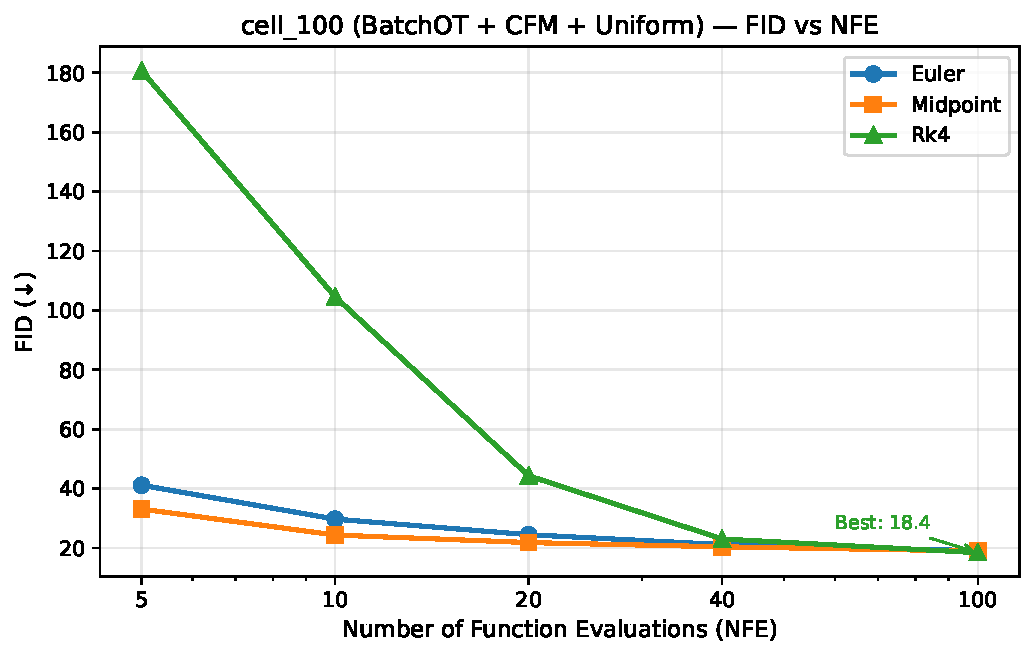
\includegraphics[width=0.65\textwidth]{figures/combined/cell_100_fid_detail.pdf}
    \caption{FID vs.\ NFE for cell\_100 (BatchOT + CFM + Uniform). Midpoint dominates at low NFE; RK4 wins at high NFE.}
    \label{fig:cell100_fid}
\end{figure}

\section{Discussion}
\label{sec:discussion}

The CIFAR-10 results are overwhelmingly negative for the variance-reduction composition hypothesis. This section analyzes each failure mode, explains the 2D-to-CIFAR gap, and answers our research questions.

\subsection{Why Cell\_000 (Baseline) Failed}

Cell\_000 uses the simplest configuration: independent coupling, standard CFM loss, and uniform timestep sampling. It diverged to NaN at step ${\sim}18{,}700$. The root cause is a numerical issue in the OT path's conditional vector field (Eq.~\ref{eq:ot_vf}):
\begin{equation}
    \ut(x | x_1) = \frac{x_1 - (1 - \sigma_{\min}) x}{1 - (1 - \sigma_{\min}) t}.
\end{equation}
The denominator $1 - (1 - \sigma_{\min}) t$ approaches $\sigma_{\min} = 10^{-4}$ as $t \to 1$. Under fp16 mixed precision, this produces values near $10^{4}$, which cascade through the network gradients and eventually overflow.

\textbf{Why BatchOT prevents this:} With independent coupling, the numerator $x_1 - (1-\sigma_{\min})x$ can be large because $x_0$ and $x_1$ are unrelated---a noise sample may be far from its paired data point. BatchOT coupling minimizes the transport cost, keeping $\|x_1 - x_0\|$ small. Since $x_t = t x_1 + \sigma_t x_0$ interpolates between paired points, both the numerator and denominator of $\ut$ remain moderate, preventing the overflow. This explains why cell\_100 converges while cell\_000 does not: BatchOT is not just a variance-reduction technique---it is a \emph{numerical stabilizer} for the OT path under limited precision.

\subsection{Why StableVM Failed}

All four StableVM cells (010, 011, 110, 111) exhibit extreme loss oscillation between ${\sim}40$ and ${\sim}22{,}000$. The cause lies in the log-probability computation (Eq.~\ref{eq:log_prob}):
\begin{equation}
    \log p_t(x | x_1) = -\frac{d}{2}\log(2\pi) - d \log \sigma_t - \frac{1}{2\sigma_t^2}\|x - \mu_t(x_1)\|^2.
\end{equation}

The critical term is $-d \log \sigma_t$. For CIFAR-10, $d = 3 \times 32 \times 32 = 3072$. Near $t = 1$, $\sigma_t \approx \sigma_{\min} = 10^{-4}$, so:
\begin{equation}
    -d \log \sigma_t \approx -3072 \times \log(10^{-4}) \approx 3072 \times 9.21 \approx 28{,}300.
\end{equation}
This enormous value dominates the softmax in the importance weights (Eq.~\ref{eq:stablevm_weights}), causing the weights to concentrate on a single reference sample---whichever $x_1^{(k)}$ is closest to $\xt$. The resulting target is effectively a single-sample estimate with high variance, but computed through a numerically unstable pathway. The loss oscillation reflects the softmax flipping between different reference samples across training steps.

\textbf{Why this is invisible in 2D:} When $d = 2$, the same term yields $-2 \times \log(10^{-4}) \approx 18.4$, which is small enough that the softmax produces meaningful weight distributions across all $K$ references. The technique works as intended in low dimensions but breaks catastrophically when $d$ is large.

\subsection{Why TPC Failed}

Cells 001 and 101 diverged to NaN at steps ${\sim}16{,}600$ and ${\sim}14{,}400$ respectively. The TPC consistency penalty (Eq.~\ref{eq:tpc_loss}) compares velocity predictions at complementary timesteps:
\begin{equation}
    \lambda \left\| \vt(\xt^{(1)}, t_1) - \vt(\xt^{(2)}, t_2) \right\|^2, \quad t_2 = 1 - t_1.
\end{equation}

When $t_1$ is close to 0 and $t_2$ close to 1, the velocity magnitudes at these two timesteps are fundamentally different: near $t=0$ the flow must move slowly from noise, while near $t=1$ it must make fine adjustments toward the data manifold. The conditional vector field magnitudes differ by orders of magnitude due to the $1/(1-(1-\sigma_{\min})t)$ denominator. The consistency penalty produces gradients that are proportional to this mismatch, leading to gradient explosions that destabilize training.

\textbf{Note:} Cell\_000 also diverged to NaN without TPC, but for a different reason (fp16 overflow from independent coupling). The NaN onset is earlier for TPC cells (14--17k steps vs.\ 18.7k), suggesting that TPC accelerates the instability.

\subsection{The 2D-to-CIFAR Gap}

All four flow-matching variants in Study~1 work perfectly in 2D, with no sign of the catastrophic failures observed on CIFAR-10. The fundamental reason is \textbf{dimensionality}:

\begin{itemize}[leftmargin=*]
    \item StableVM's log-probability scales as $O(d)$: harmless when $d=2$, catastrophic when $d=3072$.
    \item The OT path's denominator creates velocities of magnitude $\sim 1/\sigma_{\min}$. In 2D, the gradient norm stays bounded; in $d=3072$, the per-channel gradient accumulation amplifies the instability.
    \item TPC's consistency penalty couples velocities at $t$ and $1-t$ whose magnitudes diverge more severely in high dimensions, where the velocity field must navigate a higher-dimensional landscape.
\end{itemize}

This gap carries a methodological warning: \textbf{2D experiments are valuable for building geometric intuition but insufficient for validating numerical stability}. Any technique involving log-probabilities, importance weights, or time-endpoint comparisons should be stress-tested in the target dimension before deployment.

\subsection{Answering the Research Questions}

\paragraph{RQ1: Are the three axes additive?} \textbf{No.} The results are emphatically negative. Not only are the axes not additive, but combining BatchOT with either StableVM or TPC actively \emph{destroys} the convergence that BatchOT alone provides. Cell\_100 (BatchOT only) converges to FID~18.4; adding TPC (cell\_101) causes NaN divergence; adding StableVM (cell\_110) causes wild instability.

\paragraph{RQ2: Which single axis provides the largest improvement?} \textbf{BatchOT coupling}, unambiguously. It is the only axis whose inclusion leads to convergence (when used alone). StableVM and TPC both degrade performance in every tested configuration. BatchOT acts as both a variance reducer (shorter, straighter trajectories) and a numerical stabilizer (bounded velocity magnitudes).

\paragraph{RQ3: Do 2D insights transfer?} \textbf{Partially.} The geometric insight from Study~1---that OT-type paths produce straighter trajectories and better low-NFE robustness---transfers directly: cell\_100's midpoint solver at NFE=40 matches Euler at NFE=100, confirming the trajectory-straightness advantage. However, the stability insights do \emph{not} transfer: techniques that work flawlessly in 2D fail catastrophically in high dimensions.

\section{Limitations}
\label{sec:limitations}

Several design choices and constraints limit the generalizability of our findings:

\paragraph{Single seed.} All CIFAR-10 cells were trained with a single seed (seed~0). While the training failures are consistent and reproducible (all StableVM cells oscillate, all TPC cells diverge), the exact FID of the converged cell\_100 carries no error bars. Multi-seed runs would strengthen confidence in the FID=18.4 result.

\paragraph{Fast mode only.} Due to compute constraints, all cells used the fast training configuration (9M parameters, 80k steps) rather than the full configuration (47M parameters, 150k steps). While the relative comparisons remain valid (all cells share the same budget), the absolute FID of 18.4 is higher than what a fully-trained model would achieve. The failures, however, are likely to persist or worsen with longer training, since the instabilities appear early ($<20$k steps).

\paragraph{No gradient clipping.} Standard practice in diffusion/flow-matching training includes gradient norm clipping (typically to 1.0). Our training pipeline does not use gradient clipping, which likely exacerbates the NaN divergence in cells 000, 001, and 101. With gradient clipping, some of these cells \emph{might} survive longer, though the underlying numerical issues would remain.

\paragraph{fp16 mixed precision.} All training used fp16 automatic mixed precision. The OT path denominator $1-(1-\sigma_{\min})t$ reaches $10^{-4}$ near $t=1$, which is within fp16's representable range but close to its precision limit. Training in fp32 might prevent some NaN events, though at 2$\times$ memory cost.

\paragraph{Different codebases.} Study~1 and Study~2 use independent codebases with different network architectures (MLP vs.\ U-Net), optimizers (lr=$10^{-3}$ vs.\ $10^{-4}$), and data domains (2D vs.\ images). While this mirrors realistic research settings, it means that direct numerical comparisons between the two studies are not meaningful---only qualitative insights transfer.

\paragraph{CIFAR-10 only.} Results on CIFAR-10 ($32 \times 32$) may not generalize to higher-resolution datasets. The dimension-dependent failures of StableVM would only worsen at higher resolutions (e.g., $d = 3 \times 256 \times 256 = 196{,}608$ for $256 \times 256$ images).

\section{Conclusion}
\label{sec:conclusion}

We investigated whether three independently proposed variance-reduction techniques for Conditional Flow Matching---BatchOT coupling, StableVM objective, and TPC estimator---compose additively when combined. Through a $2^3$ factorial ablation on CIFAR-10, complemented by 2D synthetic experiments, we find that the answer is decisively negative.

\textbf{BatchOT coupling is the single most impactful technique.} It is the only axis whose inclusion leads to successful training (cell\_100, FID~18.4), acting simultaneously as a variance reducer and a numerical stabilizer for the OT probability path. This finding is consistent with \citet{tong2024improving} and validates BatchOT as the recommended default for CFM training.

\textbf{StableVM and TPC fail in high dimensions.} StableVM's importance weights scale with the data dimension $d$, causing softmax collapse when $d = 3072$. TPC's consistency penalty couples velocity predictions at complementary timesteps whose magnitudes differ by orders of magnitude. Both techniques work in 2D ($d=2$) but break catastrophically on CIFAR-10.

\textbf{2D experiments inform geometry but not stability.} Study~1's finding that OT-type paths produce straighter trajectories transfers to CIFAR-10 (cell\_100's solver efficiency confirms this). However, the absence of instabilities in 2D gives false confidence about numerical robustness in high dimensions.

\paragraph{Future directions.} The negative results suggest concrete remediation strategies:
\begin{itemize}[leftmargin=*]
    \item \textbf{Dimension-normalized StableVM}: Replace $\log p_t$ with $\frac{1}{d}\log p_t$ in the importance weights to prevent softmax collapse.
    \item \textbf{Gradient-stopped TPC}: Detach the consistency penalty from the computational graph to prevent gradient explosions, or restrict antithetic pairs to $t \in [0.1, 0.9]$ to avoid extreme velocity mismatches.
    \item \textbf{Gradient clipping + fp32}: Standard numerical safeguards may allow the baseline (cell\_000) and TPC cells to converge.
    \item \textbf{Multi-seed validation}: Confirm the cell\_100 result with 3--5 seeds to establish confidence intervals.
\end{itemize}

These results carry a broader methodological lesson: variance-reduction techniques should be validated not only for their statistical properties but also for their numerical stability in the target dimension. A technique that reduces variance in expectation but introduces numerical catastrophes in practice is worse than the baseline it aims to improve.


\bibliographystyle{plainnat}
\bibliography{bibliography}

\end{document}
